

%%%%%%%%%%%%%%%%%%%%%%%%%%%%%%%%%%%
\subsection{Front-end Readout and Buffering}
\label{sec:fd-daq-fero}

\metainfo{Giles Barr \& Giovanna Miotto \& Brett Viren, this is SP-specific.}

\begin{dunefigure}[Nominal \single \dword{fe} \dword{daq} fragment]{fig:daq-readout-buffering-baseline}
  {Illustration of data (solid arrows) and trigger (dashed) flow for
    one \single \dword{daq} fragment (two APAs) in the nominal design. 
    Black arrows indicate normal data and trigger flow and red indicate special flow
    for handling of a potential \dword{snb}.  } %See text for detail description.}
  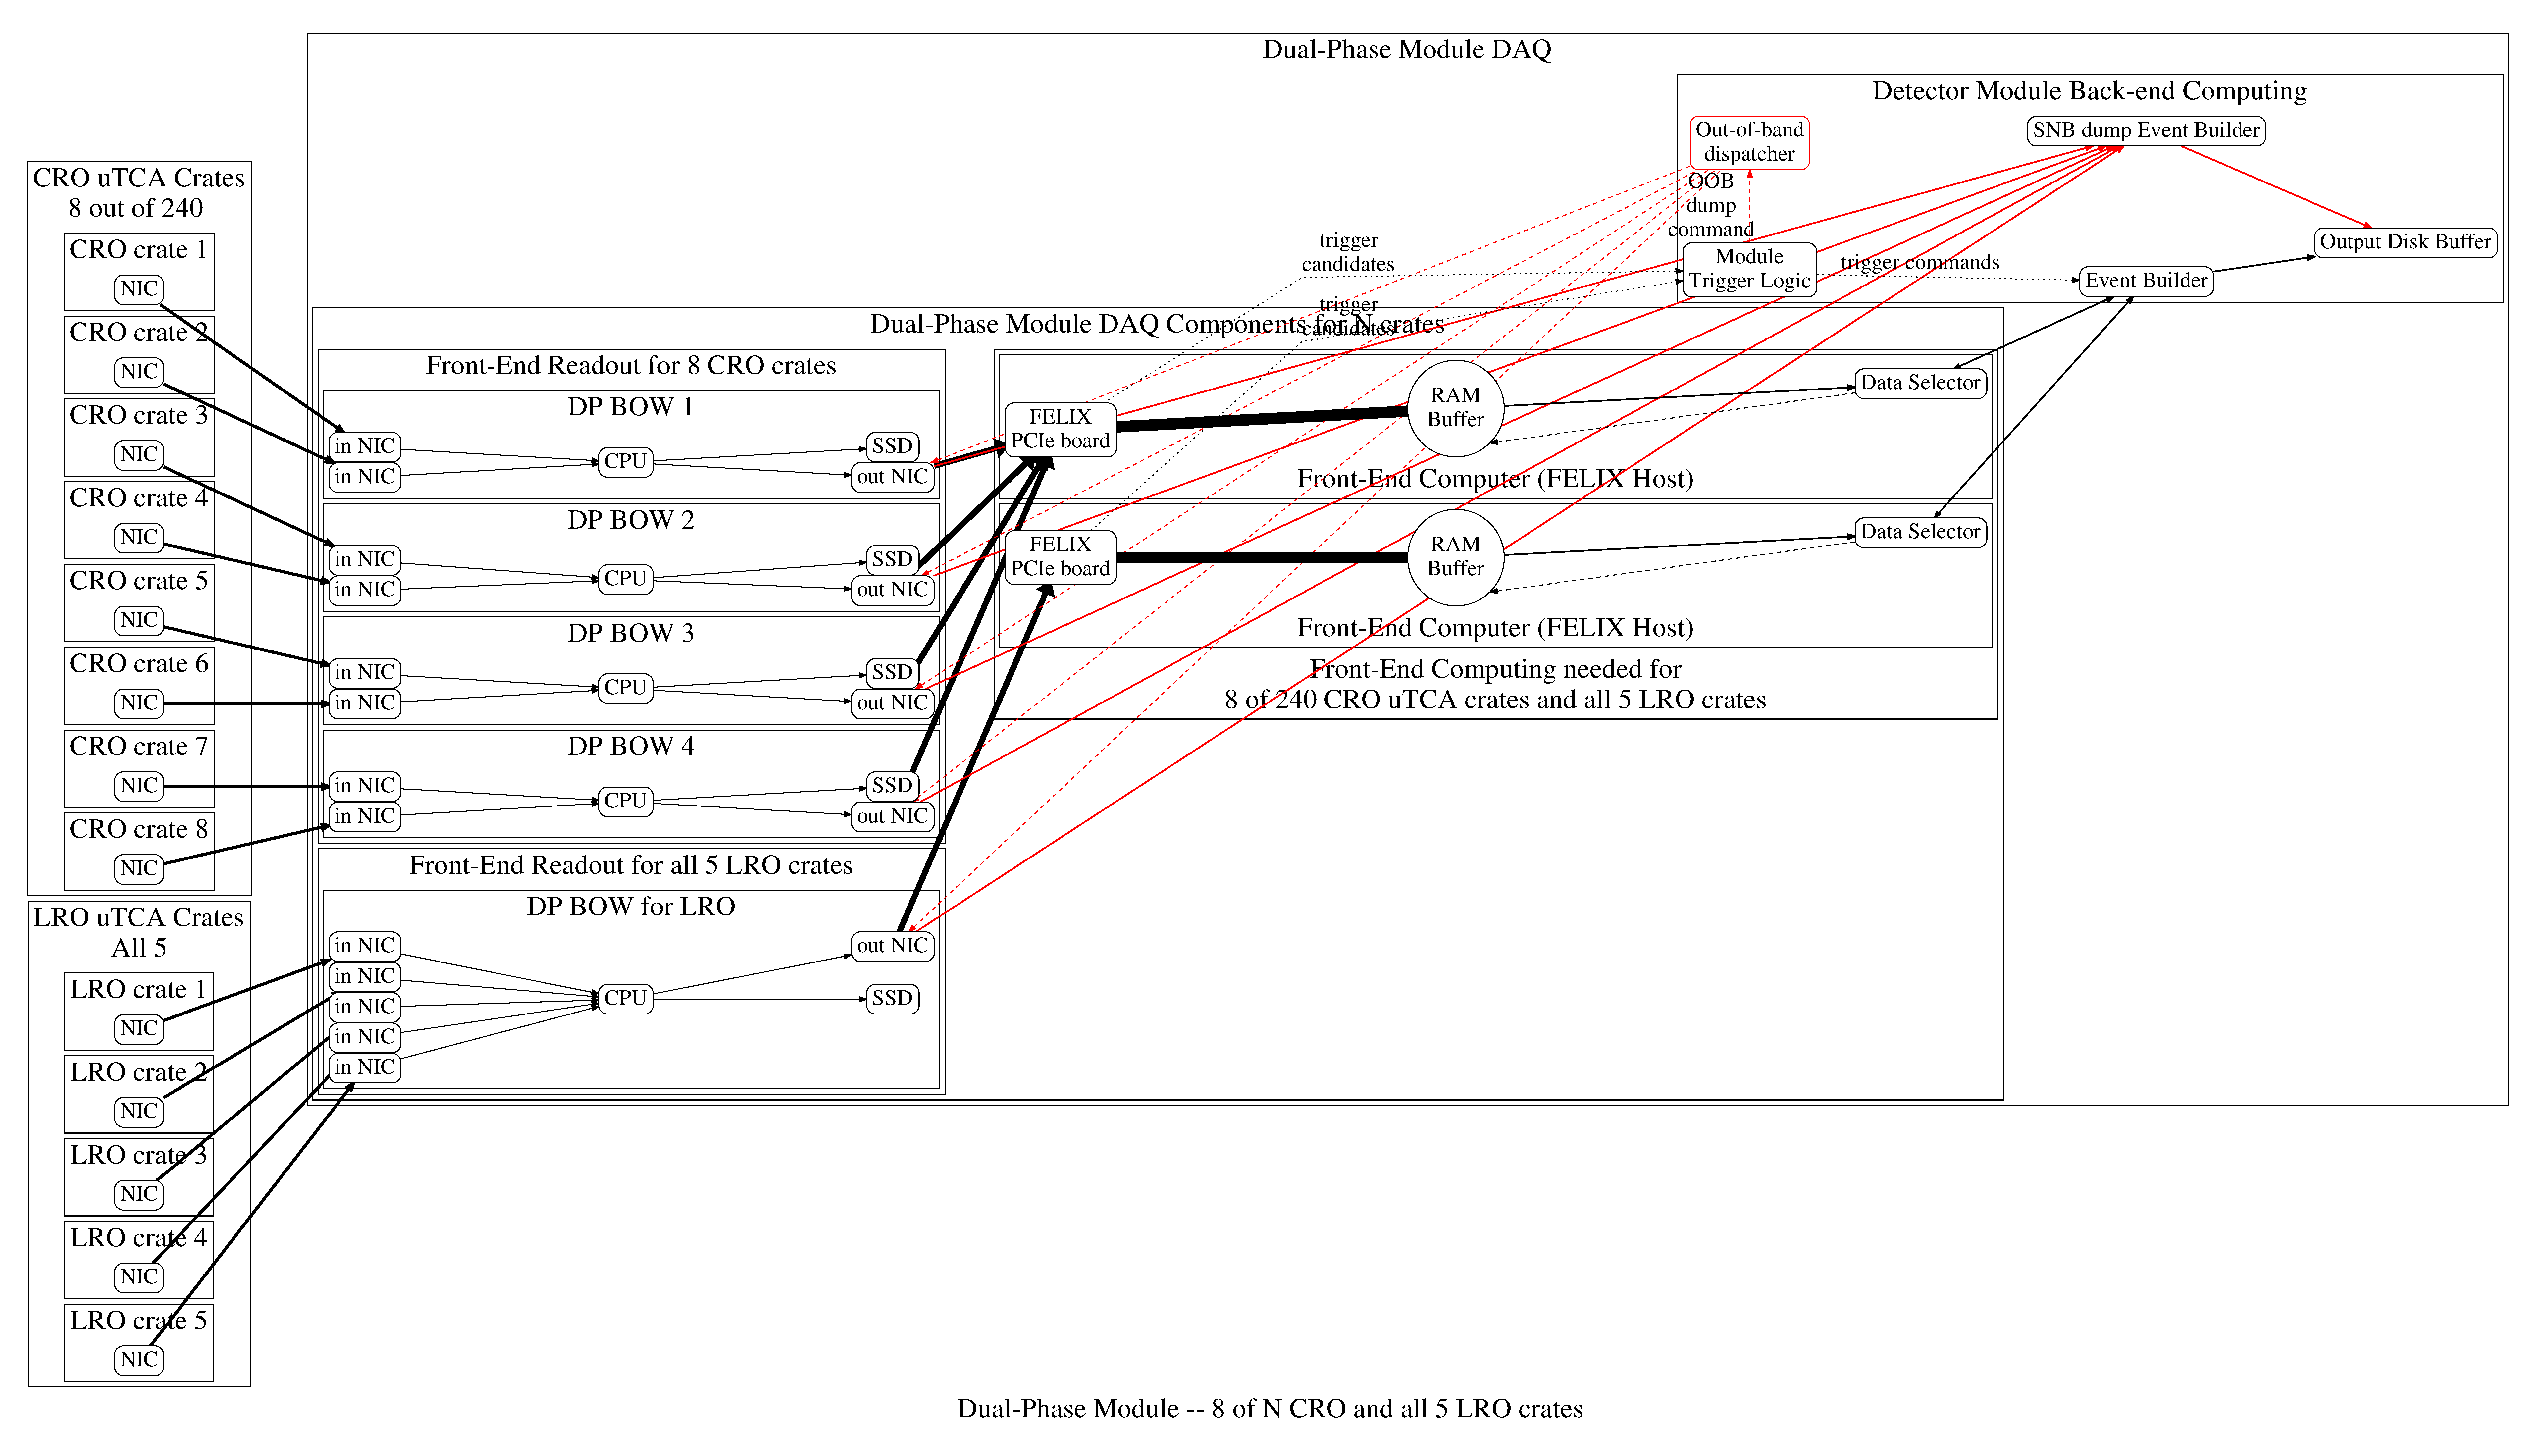
\includegraphics[width=0.95\textwidth]{daq-readout-buffering-baseline.pdf}%
\end{dunefigure}


Figure~\ref{fig:daq-readout-buffering-baseline} illustrates the
\dword{sp}-specific \dword{daqfrag} specializing from the generic,
nominal design illustrated in Figure~\ref{fig:daq-overview}.  
Starting from the left, it shows the fiber optic connectivity pattern
between the four connectors of five \dword{sp} \dwords{wib} associated
with each \dword{apa} and the elements of one \dword{sp} \dfirst{daqfer}. 
In total, the \dword{daqfer} is associated with two \dwords{apa}, each of which
is serviced by one \dshort{atca} \dfirst{cob} hosting four compute
units called \dfirst{rce}. 
Each \dword{rce} provides \dword{fpga}, RAM and \dword{ssd} resources.
Its primary functions include:
\begin{itemize}
\item Receive data from \dwords{wib},
\item Produce trigger primitives from collection channels (see Section~\ref{sec:fd-daq-fetp}),
\item Compress the data,
\item Forward data and trigger primitives to the \dword{fec},
\item Buffer data in RAM, 
\item Stream data from RAM to \dwords{ssd} on receipt of a \textit{dump}
  trigger command (such as is raised by an \dword{snb} candidate),
\end{itemize}

The data and trigger primitives from the eight \dwords{rce} are
aggregated to a single \dword{felix} PCIe board residing in the
\dword{fec}. 
This is done via \num{16} \SI{10}{\Gbps} optical fibers. 
With no data compression performed in the \dwords{rce} the bandwidth
of these fibers will be close to saturated. 
If excess noise is not greater than experienced by \microboone{}, then a
lossless compression factor of at least five may be expected.
If achieved, the total throughput into \dword{felix} from the two \dwords{apa}
is expected to be about \SI{4}{\GB/s}

The firmware running on the \dword{felix} \dword{fpga} transfers the data
and trigger streams to the host system RAM. 
This type of transfer has been demonstrated by ATLAS with a PCIe v3
\dword{felix} board at a throughput up to \SI{10}{\GB/\s}. 
The next generation of \dword{felix} based on PCIe v4 %v3 
is expected to
obtain about a factor of two improvement.
The \dwords{trigprimitive} are combined across channels to form 
\dwords{trigcandidate} that will be sent to the \dword{mtl}.
Meanwhile, the data stream streams into a \dword{daqbuf}. 
This buffer will be sized sufficient to retain the full data stream
for the period of time needed for a \dword{trigdecision} to be made. 
As described above, that decision culminates in a \dword{trigcommand}
that is sent to an \dword{eb}. 
Based on its information, the \dword{eb} makes a request to the
\dword{daqds} representing the \dword{daqfrag}, and %it 
the \dword{daqds}  replies with a 
\dword{datafrag} build from the data available in the \dword{daqbuf}.

An \dword{snb} \dword{trigcommand} is formed via the usual trigger
hierarchy, as described in %more detail in 
Section~\ref{sec:fd-daq-fetp},
and is consumed by the \dlong{daqoob} component. 
This component simply dispatches the command back down to the \num{600}
\dwords{rce} in order to relieve the duty from the \dword{mtl}, 
thus avoiding a source of trigger latency.
This means an \dword{snb} trigger command is serviced differently than
are all the other types of trigger commands. % as were described above.
The RAM on board the \dwords{rce} is used to store the full data
stream long enough for an \dword{snb} \dword{trigcommand} to be formed
and distributed. 
It has been estimated that the rise time to detect an \dword{snb} in
the \dword{sp} \dword{detmodule} is about \SI{1}{\s}, so the RAM
must be sized to buffer at least this much data.
\Dword{snb} models differ on the total duration over which significant
neutrino interactions may be expected, as well as to their possible
time profiles. 
Some allow for \dword{snb} neutrino interactions to occur for some
time but at a rate not sufficient to rise above a trigger threshold
determined by \dword{snb} backgrounds. 
It is assumed that an \dword{snb} dump should start about \snbpretime
before the \dword{snb} trigger and should span a total \snbtime.
During the dump, all data is sent to both the \dword{ssd} storage
distributed among the \dwords{rce}. 
%It 
Data also continues to flow to the associated \dword{daqfer} as during
nominal running, which ensures  that no dead time is suffered for all other
non-\dword{snb} triggers. 
The multiplicities of \dwords{rce} and \dwords{ssd} are such that
uncompressed throughput of the \dword{snb} dump will just saturate
current technology. 
Given a lossless compression factor of five the throughput to each \dword{ssd} 
is expected to be \SI{500}{\MB/\s}.

Given the infrequency of detectable \dwords{snb} the average
\dword{snb} trigger rate is effectively governed only by a chosen
threshold and by the rate of background from radiological decays,
neutrons from cosmic-ray muons and fluctuations of noise, especially
any coherent excess noise. 
The threshold must be tuned to maintain high efficiency for a broad
class of \dword{snb} models while also not flooding the \dword{daq} and
potentially offline computing. 
This needs further study, but for the purposes of illustration a
nominal false positive rate of one \dword{snb} dump per month is
assumed. 
Uncompressed, this results in \SI{540}{\TB/\year}. 
Each dump will take up \SI{75}{\GB} on an \dword{ssd}, each of which is
expected to provide \SI{500}{\GB} of storage; this is enough for
at least six dumps.
Again, lossless compression is expected to achieve a factor of five.

The \dword{snb} dumps are expected to remain on the \dword{ssd}
storage for some time in order to perform checks on the data to either
rule out and delete the data or accept the candidate and migrate its
data to permanent storage. 
This data migration is done out-of-band of the connection to the
\dword{felix} board using a local network connection to the
\dshort{atca} crate. 
With the assumed average of one dump per month, if all were saved
uncompressed it would require an average bandwidth aggregated over the
entire \dword{spmod} of just over \SI{100}{\Mbps}.

In the alternate \dword{sp} \dword{daq} design (not diagrammed), which
corresponds to the generic Figure~\ref{fig:daq-overview-alt}, the ten
\dwords{wib} shown in Figure~\ref{fig:daq-readout-buffering-baseline}
are directly connected to one \dword{felix} board via \SI{10}{\Gbps} fiber
optic.  The readout and buffering then follow the generic design.
